% Auriga theme
% https://github.com/anishathalye/auriga

\documentclass[14pt,aspectratio=169]{beamer}
\usepackage{pgfpages}
\usepackage{fancyvrb}
\usepackage{booktabs,dcolumn}
\usepackage{tikz}
\usetikzlibrary{arrows.meta, positioning, quotes}
\usepackage{pgfplots}

% \ifnotes
% \setbeamertemplate{note page}[plain]
% \setbeameroption{show notes on second screen=right}
% \fi

\usetheme{auriga}
\usecolortheme{auriga}

% define some colors for a consistent theme across slides
\definecolor{red}{RGB}{181, 23, 0}
\definecolor{blue}{RGB}{0, 118, 186}
\definecolor{gray}{RGB}{146, 146, 146}

\title{Historia Económica Argentina}

\author{\underline{Sebastián Freille} \inst{1}}

\institute[shortinst]{\inst{1} IEF-UNC \\ UCC}
\date{}

\AtBeginSection[]{
    \begin{frame}
    \vfill
    \centering
    \begin{beamercolorbox}[sep=8pt,center,shadow=true,rounded=true]{title}
        \usebeamerfont{title}\insertsectionhead\par%
    \end{beamercolorbox}
    \vfill
    \end{frame}
}



\AtBeginSubsection[]{
    \begin{frame}
    \vfill
    \centering
    \begin{beamercolorbox}[sep=6pt,center,shadow=true,rounded=true]{title}
        \usebeamerfont{title}\insertsubsectionhead\par%
    \end{beamercolorbox}
    \vfill
    \end{frame}
}


\AtBeginSubsubsection[]{
    \begin{frame}
    \vfill
    \centering
    \begin{beamercolorbox}[sep=4pt,center,shadow=true,rounded=true]{title}
        \usebeamerfont{title}\insertsubsubsectionhead\par%
    \end{beamercolorbox}
    \vfill
    \end{frame}
}


\begin{document}

{
  % rather than use the frame options [noframenumbering,plain], we make the
  % color match, so that the indicated page numbers match PDF page numbers
  \setbeamercolor{page number in head/foot}{fg=background canvas.bg}
  \begin{frame}
    \titlepage
  \end{frame}
}

  
  \section{Capítulo 3. La Economía Política del Peronismo, 1946-1955}


  \section{Inestabilidad política como contexto}
  

 \begin{frame}\frametitle{Inestabilidad política y económica}
    \begin{itemize}\itemsep 10pt
      \item Estudio de este período clave para entender el rol de la
        \textbf{inestabilidad política} en la declinación relativa de la
        economía argentina
        \item Desde 1930 del derrocamiento de Yrigoyen, hubo 7 (siete) instancias de gobiernos no democráticos
          que incluyeron episodios de gran violencia y culminaron con
          la elección democrática de Perón en 1946.
        \item Mirando en perspectiva, desde 1930 hasta la década de
          los 1990, ningún gobierno democrático pudo completar su
          mandato con excepción del primer gobierno de Perón
                 \end{itemize}
      \end{frame}



  \begin{frame}\frametitle{Inestabilidad política y económica (cont.)}
\begin{figure}[hxtbp]\vspace{0cm}
  \centering
  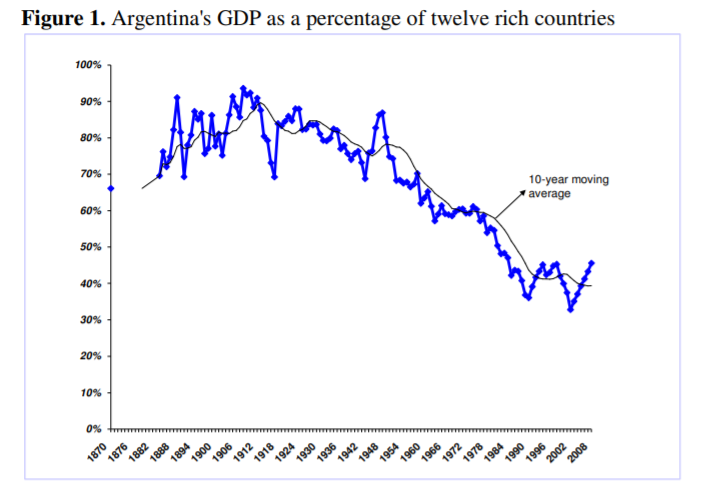
\includegraphics[scale=0.75]{uni3_contexto01}
   \label{fig:uni1_01}
\end{figure} 
  \end{frame}

           

 \begin{frame}\frametitle{Inestabilidad política y económica (cont.)}
   \begin{itemize} \itemsep 10pt
   \item El gráfico muestra el PBI de Argentina como porcentaje del
     promedio del PBI de 12 países ricos
     \item Se observa el gran desempeño de 1880-1914, la profunda y
       breve caída entre 1914-1918 y luego dos períodos márcados de
       declinación
       \item Primero, desde fines de 1920s y principios de 1930s --con
         excepción de la primera parte del gobierno de Perón y luego
         desde 1975 hasta 1990 --otro período con alta inestabilidad política
      
   \end{itemize}
          \end{frame}
  


          \begin{frame}\frametitle{Inestabilidad política y económica (cont.)}
            \begin{block}{Hipótesis}
Díaz Alejandro (1970) opina que las bajas tasas de acumulación de
capital que prevalecieron desde la Gran Depresión. Llevado a un
extremo este argumento: el mal desempeño debido a políticas populistas
implementadas por líderes que ocasionalmente explotan a una masa de
votantes pobres y con bajos niveles de educación. Problema con esta hipótesis
$\longrightarrow$ ¿por qué los votantes encuentran estas políticas
populistas atractivas? --cuestiona la efectividad de la democracia y/o
la la efectividad de los mercados [Di Tella \& Dubra (2010)]
            \end{block}               
          \end{frame}
  

\begin{frame}\frametitle{Inestabilidad política y económica (cont.)}
   \begin{itemize} \itemsep 10pt
   \item Otra hipótesis vincula a la inestabilidad política con la
     declinación económica relativa $\longrightarrow$ tasa de
     inversión durante ``década infame'' significativamente baja (9.1\%) comparada con
     promedio de siglo XX (14.4\%) y con la de 1900-1914 (19.3\%). 
         \item Hipótesis  complementaria a la de Díaz
           Alejandro --dificultad de mantener altos niveles de
           inversión cuando cambio modelo orientado a
           exportaciones a un modelo intervencionista
           \item Flujos de K y divisas
             contribuyen a aumentar la inversión, la inestabilidad
             política recurrente contribuye a desalentarla. 
   \end{itemize}
          \end{frame}
          


  \begin{frame}\frametitle{Inestabilidad política y económica (cont.)}
\begin{figure}[hxtbp]\vspace{0cm}
  \centering
  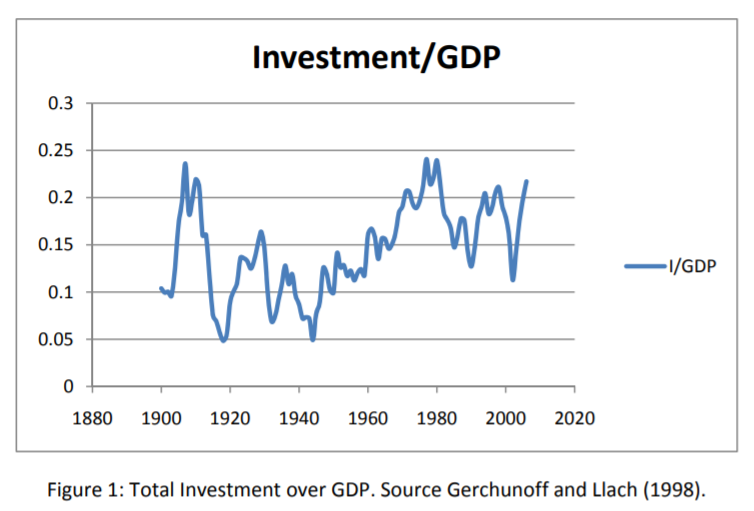
\includegraphics[scale=0.75]{uni3_contexto02}
   \label{fig:uni1_01}
\end{figure} 
  \end{frame}


    \subsection{Contexto y características de la llegada de Perón al poder}

    \begin{frame}\frametitle{Militares, política y Perón}
   \begin{itemize} \itemsep 10pt
   \item A finales de la década del 30, había una cierta esperanza de
     retomar condiciones democráticas $\longrightarrow$ elección
     \textit{fraudulenta} de
     1938 (Ortiz-UCR) aunque su prematura muerte fue un golpe a esta
     esperanza
     \item La continuidad en el poder de Ramon Castillo generaba
       fricciones $\longrightarrow$ posición de política exterior
       argentina (2GM) y fricciones con eje militar-nacionalista
       \item Las renuncias de los liberales Roca y Pinedo --funcionarios de
         Castillo- terminaron de definir el destino de la posición argentina
   \end{itemize}
          \end{frame}
          

 \begin{frame}\frametitle{Militares, política y Perón (cont.)}
   \begin{itemize} \itemsep 10pt
   \item Argentina mantuvo neutralidad y trató de conservar una
     política de autonomía en terminos internacionales (lo que no caía
     bien en EEUU)
     \item Gradual politización de las Fuerzas Armadas
       $\longrightarrow$ Grupo de Oficiales Unidos (GOU) --mantener
       neutralidad, impedir ideas comunistas y posicionar a militares
       como elemento estabilizador
       \item Luego de una serie de desacuerdos entre el Gobierno de
         Castillo y militares, sobrevino la decisión del golpe de
         estado de 1943. 
   \end{itemize}
          \end{frame}



 \begin{frame}\frametitle{Militares, política y Perón (cont.)}
   \begin{itemize} \itemsep 10pt
   \item La revolución del 43 tuvo como principal (y único?) objetivo
     derrocar al Presidente --Pedro Ramírez ocupa el cargo pero fue
     influenciado por el GOU (general Farrel y coroneles como Perón)
          \item Los dos ejes políticos centrales antes de 1946 fueron:
            1) ascenso de Perón, 2) posición argentina sobre 2GM
            \item Perón acumulaba cargos --ministro de Guerra,
              sec. de Trabajo y Previsión y vicepres- y
               ambiciones políticas
              \item En relación a 2GM, mayores tensiones con EEUU dado
                que Argentina no rompía con potencias del
                Eje 
   \end{itemize}
 \end{frame}


  \begin{frame}\frametitle{El tercer sacudón en 30 años: la 2GM}
   \begin{itemize} \itemsep 10pt
   \item La 2GM agarra a la Argentina en plena recuperación post-Gran
     Depresión --el PBI crecía al 4\% entre 1933 y 1939. Pero debajo
     de esa superficie, había cambios profundos: 1) nuevas
     instituciones (BCRA, controles cambiarios, juntas reguladoras) y
     2) presencia industrial sólida
     \item El propósito del Plan Pinedo de 1940 fue esencialmente un
       intento de minimizar los efectos de la ola proteccionista sobre
       la economía nacional $\longrightarrow$ fracaso del PP por
       razones políticas y previsiones pesimistas
   \end{itemize}
          \end{frame}



  \begin{frame}\frametitle{El tercer sacudón en 30 años: la 2GM (cont.)}
\begin{figure}[hxtbp]\vspace{0cm}
  \centering
  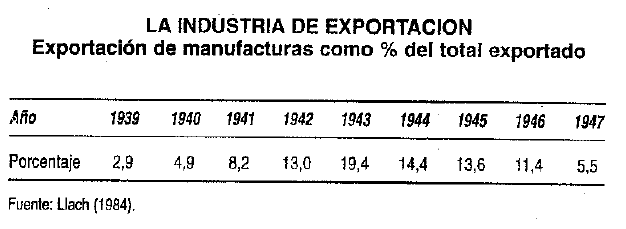
\includegraphics[scale=0.75]{uni3_contexto03}
   \label{fig:uni1_01}
\end{figure} 
  \end{frame}


 \begin{frame}\frametitle{El tercer sacudón en 30 años: la 2GM (cont.)}
   \begin{itemize} \itemsep 10pt
   \item Entre 1939 y 1944 el crecimiento fue de 3.6\% (1939-1945,
     2.5\%). La producción creció al amparo de la industria y se
     exportaron manufacturas a otros países (Brasil, EEUU).
   \item Este efecto vino principalmente impuesto por condiciones
     externas --economía de guerra, proteccionismo y sustitución de M
     \item A pesar del buen desempeño relativo entre 1939 y 1945, el
       crecimiento fue menor que otros países de Latam y que EEUU y
       Canadá. 
   \end{itemize}
          \end{frame}

  

  \begin{frame}\frametitle{El tercer sacudón en 30 años: la 2GM (cont.)}
\begin{figure}[hxtbp]\vspace{0cm}
  \centering
  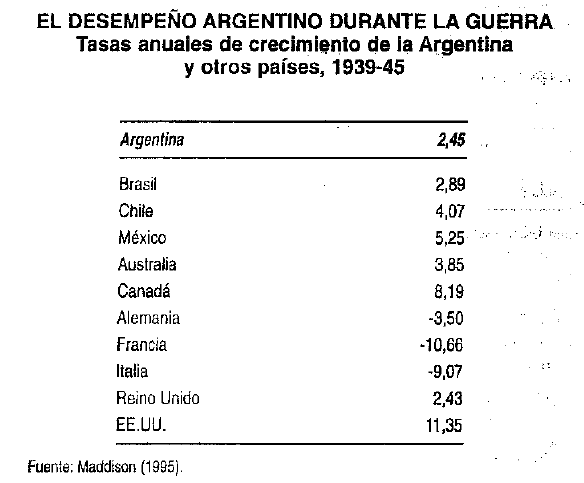
\includegraphics[scale=0.75]{uni3_contexto04}
   \label{fig:uni1_01}
\end{figure} 
  \end{frame}

          



 \begin{frame}\frametitle{El tercer sacudón en 30 años: la 2GM (cont.)}
   \begin{block}{}
       
Si alguien hubiese preguntado en 1945 ¿qué parte del mundo espera
usted que experimente el más dramático despegue económico en las
próximas tres décadas?, probablemente yo habría dado una respuesta
parecida a la siguiente: la Argentina es la ola del futuro, tiene
clima templado, su densidad de población ofrece una dotación favorable
de recursos naturales por empleado. Por un accidente histórico, su
población actual constituye la más homogénea progenie de las naciones
de Europa Occidental y la Argentina en 1945 se encuentra en ese estado
intermedio de desarrollo del cual se puede fácilmente esperar un
rápido crecimiento [Paul Samuelson]
     \end{block}
                 \end{frame}
  


\begin{frame}\frametitle{La hora del industrialismo (?)}
   \begin{itemize} \itemsep 10pt
   \item Idea de promover la industrialización a través de políticas
     estatales no era nueva $\longrightarrow$ Pellegrini, V. Lopez,
     Bunge entre otros alertaban sobre necesidad de desarrollar
     industria
     \item Hasta 1930 Argentina no era más proteccionista que otros
       países avanzados (EEU, Australia, Canadá) --medidas respondían
       a necesidad recaudatoria, evitar drenaje de reservas y a
       presiones de lobby
       \item No hubo política consciente y coherente de fomento a la
         industria [volveremos a este punto] 
   \end{itemize}
 \end{frame}
                 


\begin{frame}\frametitle{La hora del industrialismo (?) (cont.)}
   \begin{itemize} \itemsep 10pt
   \item Entre 1940 y 1943 $\longrightarrow$ redescuentos del BCRA
     asimétricos, leyes de promoción industrial regionales, ley de
     Fabricaciones Militares
     \item Opinión favorable general sobre apoyo a industria admitía
       debates $\longrightarrow$ industrias naturales (Pinedo) vs
       artificiales [UIA promovía industrialización a todo nivel]
          \item Otro debate $\longrightarrow$ ¿producir para mercado
            interno o externo? --industrialización para la liberación
            económica y autonomía nacional [Castillo]            
   \end{itemize}
 \end{frame}
             
 
\begin{frame}\frametitle{La hora del industrialismo (?) (cont.)}
   \begin{itemize} \itemsep 10pt
   \item Consignas nacionalistas en el corazón del pensamiento
     pro-industrial $\longrightarrow$ hizo fuerte eco en las Fuerzas
     Armadas (Ejército)
     \item Inicialmente, se orientó a industria bélica y relacionada;
       luego se extendió a otras industrias (basada en la importancia
       de la defensa nacional)
       \item De este modo, coincidían dos grandes actores emergentes
         en décadas recientes --UIA y Fuerzas Armadas
   \end{itemize}
 \end{frame}

 
\begin{frame}\frametitle{La hora del industrialismo (?) (cont.)}
   \begin{itemize} \itemsep 10pt
   \item Inicialmente, Consejo Nacional de Posguerra (auspiciado por Perón) tenía línea
     moderada a la Pinedo (``industrialización razonable'')
     \item Con los años, Perón cambiaría --para él, la importancia de
       la industrialización no tenía que ver con el nacionalismo sino
       como parte de un eje mucho más económico --nivel de empleo y
       ocupación
       \item Con el fin de la 2GM, muchas actividades desaparecerían
         en ausencia de apoyo estatal --sus aspiraciones políticas no
         podían permitir la pérdida del apoyo de trabajadores industriales
   \end{itemize}
 \end{frame}



  \begin{frame}\frametitle{La hora del industrialismo (?) (cont.)}
\begin{figure}[hxtbp]\vspace{0cm}
  \centering
  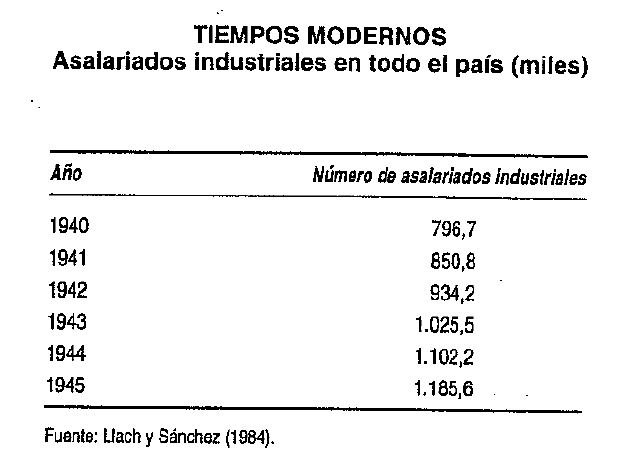
\includegraphics[scale=0.75]{uni3_contexto05}
   \label{fig:uni1_01}
\end{figure} 
  \end{frame}


\begin{frame}\frametitle{Reflexiones desde la teoría}
   \begin{itemize} \itemsep 10pt
   \item Muchos autores ven en las políticas económicas del primer
     peronismo el resultado de una alianza (coalición) deliberada y
     explícita entre el gobierno y sectores sociales --principalmente,
     sindicatos (Iglesia, militares). Consecuencia de ello fue una
     asignación ineficiente de recursos que profundizó un sesgo
     anti-exportador presente en Argentina desde el final de la 2GM
          \item Hipótesis alternativa $\longrightarrow$ entre 1946 y
            1955 no existió una política económica ``peronista'' específica y
            unificada ni mucho menos un plan de desarrollo de largo plazo
   \end{itemize}
 \end{frame}


\begin{frame}\frametitle{Reflexiones desde la teoría (cont.)}
   \begin{itemize} \itemsep 10pt
   \item Más allá de la retórica sobre planes y programas, el objetivo
     prioritario fue una rápida modificación en la distribución del
     ingreso en beneficio de los trabajadores seguido de un orden
     económico que pudiera sustentar el nuevo modelo distributivo
     \item Este objetivo y su celeridad requiere de una subordinación
       de la economía a la política, una aumentada intervención
       estatal
       \item Esto no es necesariamente algo particular y/o específico
         del peronismo $\longrightarrow$ pasaba en la posguerra y en
         nuestros días
   \end{itemize}
 \end{frame}




\begin{frame}\frametitle{Reflexiones desde la teoría (cont.)}
   \begin{itemize} \itemsep 10pt
   \item Lo que hizo distintivo al peronismo en este sentido fue la
     intensidad de la ``primacía de la política'' $\longrightarrow$
     incluyó a los trabajadores industriales (organizados) como parte esencial
     (sustento electoral) de la
     coalición de gobierno
     \item Esta coalicíon no incluyó por defecto a trabajadores
       rurales ni empresarios y comerciantes
       \item Un efecto de la dominancia de la política fue la
         expansión del Estado y el aumento de controles y regulación
\end{itemize}
       \end{frame}



 
\begin{frame}\frametitle{Reflexiones desde la teoría (cont.)}
   \begin{itemize} \itemsep 10pt
   \item Podemos tal vez realizar una tentativa interpretación de la
     economía-política subyacente de algunos de estas estrategias y
     lineamientos de política
     \item Usando las herramientas de la economía-política y modelos
       sencillos de impuestos y gastos con votantes, es posible
       acercarse a entender cómo estas políticas pueden ser
       contextualizas en un marco de racionalidad de agentes.
\end{itemize}
     \end{frame}



\begin{frame}\frametitle{Reflexiones desde la teoría (cont.)}
\begin{itemize}
\item Suponga un gobierno que debe decidir el nivel de gasto e
  imposición. Existe un sólo impuesto $\longrightarrow$ el impuesto a
  la renta. Debe determinarse la alicuota, $\tau$. Si el ingreso
  individual es $y$, el ingreso después de impuestos es $y(1-\tau)$.
\item La imposición tiene un costo. Supongamos que el costo
  (distorsión) del impuesto es igual a $\delta \tau^2$. 
\item El votante mediano quiere maximizar su consumo (depende del
  ingreso después de impuestos, del gasto público y del costo de la
  imposición).
\end{itemize}
\end{frame}
     


     \begin{frame}\frametitle{Reflexiones desde la teoría (cont.)}
\begin{itemize}\itemsep 15pt
\item El consumo final de un persona viene dado por:
\begin{equation}
C=y(1-\tau)+\tau y_{avg}-\delta \tau^2
\end{equation}
\item y la alícuota óptima viene dada por:
\begin{equation}
\tau=\frac{y_{avg}-y_{median}}{2\delta}
\end{equation}
\item Note que la \textit{alícuota (y el tamaño del gobierno) son crecientes
  en la \underline{diferencia} entre el ingreso promedio y el ingreso mediano}. 
\item Clave $\longrightarrow$ políticos toman decisiones
  basadas en votante mediano; tasas
  medias están basadas en el ingreso medio. 
\end{itemize}
\end{frame}


\begin{frame}\frametitle{Reflexiones desde la teoría (cont.)}
\begin{itemize}
\item Suponga 5 personas (y suponga $\delta=0.5$). Sea $y={0,1,2,3,4}$
\begin{itemize}\itemsep 0pt \medskip
\item Mediana? 2 ---  Media? 2 --- $\tau$? 0
\item $C=y(1-\tau)+\tau y_{avg}-\delta \tau^2$ $\Rightarrow$ $C=2(1-0)+0-0=2$
\end{itemize}
\item Ahora, con $y={0,1,2,3,9}$
\begin{itemize}\itemsep 0pt \medskip
\item Mediana? 2 --- Media? 3 --- $\tau$? 1
\item $C=y(1-\tau)+\tau y_{avg}-\delta \tau^2$ $\Rightarrow$ $C=2(1-1)+1*3-0.5=2.5$
\end{itemize}
\item Ahora, con $y={0,1,2,3,59}$
\begin{itemize}\itemsep 0pt \medskip
\item Mediana? 2 --- Media? 13 --- $\tau$? 11
\item $C=y(1-\tau)+\tau y_{avg}-\delta \tau^2$ $\Rightarrow$ $C=2(1-11)+11*13-0.5*(11)^2=62.5$
\end{itemize}
\end{itemize}
\end{frame}


\begin{frame}\frametitle{Reflexiones desde la teoría (cont.)}
\begin{itemize}
\item ¿Qué esta ocurriendo? 
\begin{itemize}
\item Lo que sucede es que en este simple modelo \textit{la política está determinada por la
  diferencia entre el mediano y la media}
\item Esto implica que, por ejemplo, cuando existen grandes niveles de
  desigualdad (particularmente cuando hay personas extremadamente
  ricas como en el tercer caso), el votante mediano puede ganar mucho
  al fijar una alícuota mayor y poner impuestos sobre los ricos. 
\end{itemize}
\item ¿Por qué la alícuota era igual a cero en el caso 1 cuando el
  mediano y la media eran iguales?
\begin{itemize}\itemsep 5pt \medskip
\item El mediano no se beneficia en absoluto de que haya una alícuota
  (ver consumo). Como la imposición es costosa (distorsiva), la
  alícuota optima es igual a 0. 
\end{itemize}
\end{itemize}
\end{frame}


\begin{frame}\frametitle{Reflexiones desde la teoría (cont.)}
\begin{block}{Utilidad del teorema del votante mediano}
We appeal to this (median voter) theorem to capture the basic idea that
any government is likely to be responsive to the wishes of the majority when
key distributional issues are at stake. Even a dictator cannot completely
ignore social demands for fear of being overthrown. Thus, even in a
dictatorship, distributional issues affecting the majority of the population
will influence policy outcomes [Alesina and Rodrik (1994)]
\end{block}
\end{frame}



 \section{Perón: ascenso al poder. Sus ideas económicas, políticas
   y sociales}
  

\begin{frame}\frametitle{Perón en el poder: Economía y política}
   \begin{itemize} \itemsep 10pt
   \item Entre la revolución de 1943 y 1946, Perón fortaleció sus
     lazos con el poder sindical $\longrightarrow$ asume el
     Dpto Nacional de Trabajo y luego la Secretaría de Trabajo y Previsión. 
     \item Inmediatamente reconoce la conveniencia de mutar de una
       política de control/dominación a sindicatos a una de
       diálogo/concesiones
       \item Da concesiones a (e intercede a favor de) varios sectores
         --ferroviarios; en general a través de aumentos salariales y
         salarios mínimos (sistema de precios) y no a través de
         redistribución (impuesto/gasto)
   \end{itemize}
 \end{frame}


 

 \begin{frame}\frametitle{Perón en el poder: Economía y política (cont.)}
   \begin{itemize} \itemsep 10pt
   \item Empieza así a forjarse aún antes de la presidencia de Perón
     una alianza de sindicatos con el Gobierno --pragmatismo de ambos
     lados
     \item En 1945, acicalado por el apoyo sindical y por los sectores
       nacionalistas, Perón era la figura pública más importante del
       país --lo que generó protestas desde sectores con ideal republicano
       \item En octubre de 1945, Perón renuncia a todos sus cargos y
         luego es arrestado $\longrightarrow$ movilización popular
         (gremios+trabajadores) del 17 de octubre forzó la mano
         definitivamente a favor de Perón 
   \end{itemize}
 \end{frame}


  \begin{frame}\frametitle{Perón en el poder: Economía y política (cont.)}
   \begin{itemize} \itemsep 10pt
   \item Perón gana las eleccionnes democráticas de 1946 sobre la
     Unión Democrática (``Braden o Perón'') por amplio margen
     $\longrightarrow$ apoyo electoral de sindicatos, Iglesia y
     militares
   \item Tríptico de sustento de poder:
     \begin{itemize}\itemsep 10pt \medskip
     \item Sindicatos $\longrightarrow$ ``el ejército que produce''
     \item Militares $\longrightarrow$ ``el ejército que cuida''
       \item Iglesia $\longrightarrow$ ``fuente del poder moral''
       \end{itemize}
        \item Un rasgo inmutable en la concepción de Perón fue la
          visión corporativista $\longrightarrow$ mayores beneficios
          fueron siempre para trabajadores sindicalizados (no para los
          no agremiados)
   \end{itemize}
 \end{frame}


  \begin{frame}\frametitle{Perón en el poder: Economía y política (cont.)}
    \begin{block}{Visión corporativista}
      Los gremios más beneficiados, los que han visto acumular en su
      favor el mayor número de conquistas, son los gremios mejor
      organizados. Esto quiere decir que la Secretaría de Trabajo y
      Previsión cumple conscientemente con su deber, escuchando el
      clamor de los trabajadores organizados, recibiendo la
      manifestación de sus aspiraciones colectivas, porque tienen más
      facilidad para hacerse oir las organizaciones series, estables y
      responsables, porque tienen más acierto en el reclamo de sus reinvidicaciones...
      \end{block}
 \end{frame}



  \begin{frame}\frametitle{Perón en el poder: Economía y política (cont.)}
   \begin{itemize} \itemsep 10pt
   \item Perón se esforzó por distanciarse del pensamiento de
     izquierda. Propuso ``armonía de clases'' en contraposición a la
     ``lucha de clases'' $\longrightarrow$ ``ni comunista ni
     capitalista, justicialista''
     \item Su filosofía económica lejos de ser dogmática era más bien
       pragmática $\longrightarrow$ eclecticismo oportuno para
       resolver dilemas distributivos 
\item Durante varios años (bonanza post guerra) la alianza obreros-empresarios industriales
  pudo mantener una armonía --pero esto pronto sería fuente de tensiones
     \end{itemize}
 \end{frame}


  \begin{frame}\frametitle{Perón en el poder: Economía y política (cont.)}
   \begin{itemize} \itemsep 10pt
   \item No sólo en temas distributivos el peronismo fue promotor de
     una posición intermedia (``tercera vía'') --sino que también en
     la política internacional
     \item Perón veía posible una 3GM y un agravamiento de las
       tensiones comerciales $\longrightarrow$ habilita la opción de
       la autarquía económica y el mercado-internismo
       \item RRII con EEUU y UK mezcla de nacionalismo con sentido de
         oportunidad $\longrightarrow$ exclusión argentina del Plan
         Marshall un castigo a la indiferencia argentina
     \end{itemize}
 \end{frame}


  \begin{frame}\frametitle{Perón en el poder: Economía y política (cont.)}
   \begin{itemize} \itemsep 10pt
   \item Una cuestión muy delicada fue la negociación con UK para el
     arreglo de las cuentas de guerra. Se pasó de una BP relativamente
     equilbrada a una BP fuertemente superativaria de Argentina
     \item UK tenía una fuerte deuda de más de 100 millones de libras
       --''libras bloqueadas'' ya que eran inconvertibles con el
       dolar. Gran perjuicio para Argentina que comerciaba mucho con EEUU
       \item Acuerdo final --ferrocarriles y libras bloqueadas: se
         usaron para comprar los FFCC [opiniones divididas]
     \end{itemize}
   \end{frame}


   \begin{frame}\frametitle{Perón en el poder: Economía y política (cont.)}
   \begin{itemize} \itemsep 10pt
   \item Una cuestión muy delicada fue la negociación con UK para el
     arreglo de las cuentas de guerra. Se pasó de una BP relativamente
     equilbrada a una BP fuertemente superativaria de Argentina
     \item UK tenía una fuerte deuda de más de 100 millones de libras
       --''libras bloqueadas'' ya que eran inconvertibles con el
       dolar. Gran perjuicio para Argentina que comerciaba mucho con EEUU
       \item Acuerdo final --ferrocarriles y libras bloqueadas: se
         usaron para comprar los FFCC [opiniones divididas]
     \end{itemize}
 \end{frame}
 
                 
\end{document}

      